\chapter{系统设计}

\section{总体设计}

本系统总体上采用前后端分离的微服务化分层架构设计（Layered Architecture），并结合大语言模型组件和检索引擎进行了特化。总体架构自下而上分为基础设施层、数据持久层、业务服务层及表现层，同时引入了 AI Agent 中间件来桥接数据层与表现层。

\begin{figure}[ht]
  \centering
  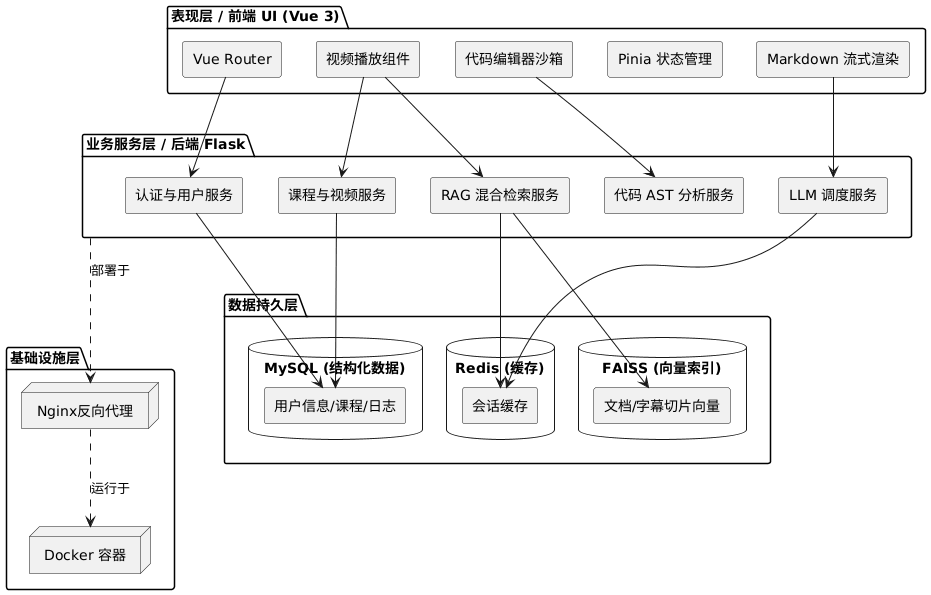
\includegraphics[width=\textwidth,height=0.4\textheight,keepaspectratio]{arch.png} % 架构图
  \caption{基于大模型的个性化学习系统分层架构实例}
  \label{fig:architecture}
\end{figure}

系统架构特化描述如下：

（1）\textbf{基础设施层}：通过 Docker 容器化部署在 Linux 服务器上，由 Nginx 进行动静分离及反向代理，有效提升了前端静态资源的加载速度。

（2）\textbf{数据持久层}：采用多源存储架构。MySQL 用于存储强一致性的结构化业务数据；Redis 作为内存中间件，缓存频繁访问的数据及维护问答会话的上下文；FAISS 向量数据库用于持久化存储视频字幕与教案的稠密语义向量。

（3）\textbf{业务服务层（核心层）}：在 Flask 后端框架上，划分为基础业务逻辑（认证、课程管理）和 AI 增强引擎（RAG Retrieval Pipeline，代码 AST Static Analyzer，LLM Invocation Service）。该层通过消息队列或线程池异步调度高负载的预处理任务。

（4）\textbf{表现层}：基于 Vue 3 构建的富客户端应用，实现了与用户的强交互，包括流式 Markdown 渲染、Markdown 到视频时间轴的事件联动以及动态渲染的在线代码编辑器沙箱。

\section{详细设计}

详细设计主要包括核心模块的类与时序设计、数据库结构（E-R 图）、接口规范以及关键界面设计。

\subsection{模块/类设计}

以“启发式代码提交与评测”这一核心模块为例，以下给出该模块的时序图。该图展示了从前端发起提交，到后端协调代码静态分析器、生成提示词、调用大语言模型服务，最后流式响应反馈给前端的整个交互生命周期。

\begin{figure}[ht]
  \centering
  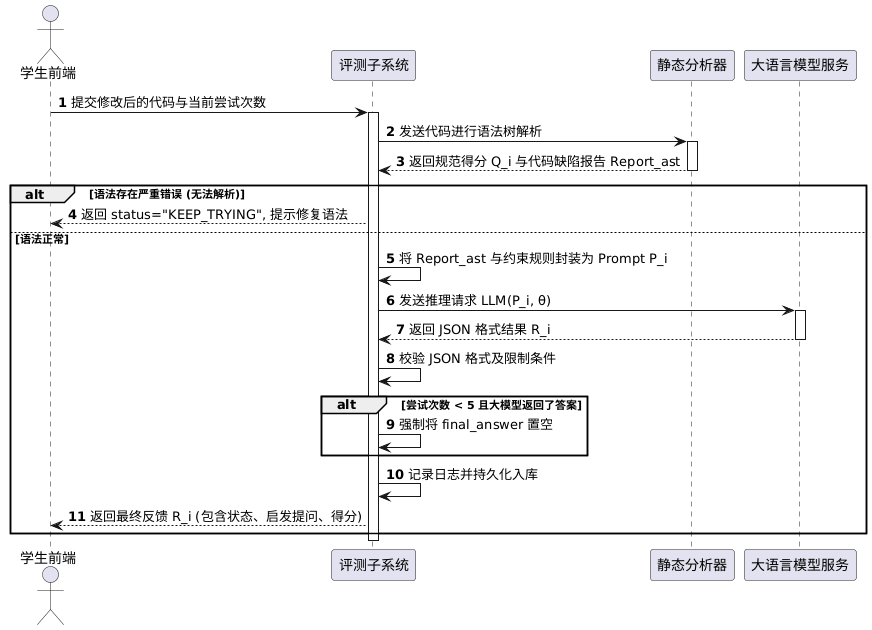
\includegraphics[width=\textwidth,height=0.4\textheight,keepaspectratio]{sequence.png} % 时序图
  \caption{“启发式代码提交与评测”用例实现的时序图}
  \label{fig:sequence_code_eval}
\end{figure}

\subsection{数据库设计}

为了支撑系统的多模态数据与学习者的状态记录，需要对核心实体及其关联进行详细建模。系统的主要实体包括：用户（User）、课程（Course）、视频资源（Video）、问答会话（ChatSession）、对话消息（Message）以及代码评测记录（CodeTaskRecord）。

\begin{figure}[ht]
  \centering
  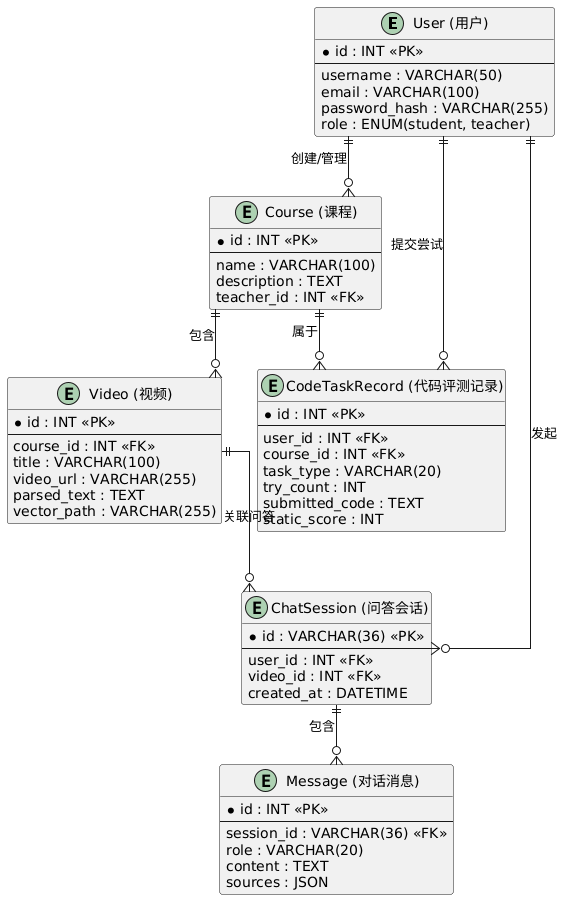
\includegraphics[width=\textwidth,height=0.4\textheight,keepaspectratio]{er.png} % ER图
  \caption{在线个性化学习系统 E-R 图}
  \label{fig:er_diagram}
\end{figure}

\textbf{主键与多重性分析}：

（1）\textbf{User 与 Course (1对多)}：一个教师（Teacher 角色）可以创建并管理多门课程，\texttt{teacher\_id} 作为 Course 表的外键\cite{whu-bachelor:28}。

（2）\textbf{Course 与 Video (1对多)}：一门课程下挂载多个教学视频。Video 表除了基本的自增主键 \texttt{id}外，还包含外键 \texttt{course\_id}。

（3）\textbf{ChatSession 与 Message (1对多)}：每一个问答会话包含多条流式对话消息，Message 表中的 \texttt{session\_id} 关联至 ChatSession 的主键。

\textbf{数据库核心表结构详述}：
\begin{table}[ht]
\centering
\caption{User (用户表) 设计}
\label{tab:user_table}
\begin{tabular}{|l|l|l|p{5cm}|}
\hline
字段名 & 数据类型 & 约束 & 描述 \\ \hline
id & INT & PRIMARY KEY, AUTO\_INC & 用户唯一标识 \\ \hline
username & VARCHAR(50) & NOT NULL, UNIQUE & 用户登录名 \\ \hline
email & VARCHAR(100) & NOT NULL, UNIQUE & 注册邮箱 \\ \hline
password\_hash & VARCHAR(255) & NOT NULL & 加盐哈希后的密码 \\ \hline
role & ENUM & DEFAULT 'student' & 角色类型(student/teacher) \\ \hline
\end{tabular}
\end{table}

\begin{table}[ht]
\centering
\caption{Video (视频资源表) 设计}
\label{tab:video_table}
\begin{tabular}{|l|l|l|p{5cm}|}
\hline
字段名 & 数据类型 & 约束 & 描述 \\ \hline
id & INT & PRIMARY KEY, AUTO\_INC & 视频记录主键 \\ \hline
course\_id & INT & FOREIGN KEY & 归属的课程ID \\ \hline
title & VARCHAR(100) & NOT NULL & 视频标题 \\ \hline
video\_url & VARCHAR(255) & NOT NULL & 视频文件存储路径或OSS地址 \\ \hline
parsed\_text & TEXT & NULL & ASR解析生成的完整字幕 \\ \hline
vector\_path & VARCHAR(255) & NULL & 对应的FAISS向量库索引路径 \\ \hline
\end{tabular}
\end{table}

\subsection{接口设计}

系统采用 RESTful 风格的 API 设计规范。以下列举并详细说明两个关键接口。

\textbf{1. 生成智能代码实训题目接口}

\textbf{URL}：\texttt{/api/code\_training/generate\_task} \\
\textbf{Method}：POST \\
\textbf{描述}：根据指定的课程范围与任务类型（Debug 或 Refactor），通过大语言模型动态生成包含预设缺陷或坏味道的代码模板及题目描述\cite{whu-bachelor:20}。在数学模型上，可将生成任务抽象为函数 $G(k, t) \rightarrow \{id, D, C_{bad}\}$，其中 $k$ 为知识点范畴约束，$t \in \{debug, refactor\}$ 为任务类别。 \\
\textbf{请求参数}：
（1）\texttt{keyword} (String, 必填)：限定题目的知识点范畴。
（2）\texttt{task\_type} (String, 选填)：任务类别。 \\
\textbf{响应结构}：系统返回格式化的键值对数据，包含任务的唯一标识 $id$、任务类别描述、以及由模型构造的带有特定逻辑漏洞的原始代码段 $C_{bad}$，供前端渲染到沙箱中供学生作答。

\vspace{1em}
\textbf{2. 视频资源 AI 流式问答接口}

\textbf{URL}：\texttt{/api/qa/ask-stream} \\
\textbf{Method}：POST \\
\textbf{描述}：基于 SSE（Server-Sent Events）的检索增强流式问答，前端通过 EventSource 持续接收输出流，实现打字机效果。可以表示为连续的 token 序列输出 $S = \{w_1, w_2, \dots, w_n\}$，其中 $w_i$ 随时间 $T_i$ 逐步抵达客户端\cite{whu-bachelor:30}。 \\
\textbf{请求参数}：
（1）\texttt{question} (String, 必填)：用户的自然语言提问。
（2）\texttt{videoIds} (Array, 选填)：限定在特定视频的上下文切片中进行检索。
（3）\texttt{session\_id} (String, 选填)：用于维持多轮对话记忆的唯一标识符。 \\
\textbf{返回机制}：通过 \texttt{text/event-stream} 协议头，分块返回大模型生成的答案及溯源引用标记数据。

\subsection{界面设计}

系统的界面设计注重用户的沉浸感与交互反馈，以下为两个核心界面的原型设计说明。

\textbf{智能代码实训工作台原型}：
界面左侧为任务描述区与 AI 导师反馈区。上方包含“获取 Debug 专项题”与“获取代码质量重构题”两个高亮按钮；中间展示任务的详细文本；下方则为一个动态的“状态徽章”卡片，用于显示大模型的启发评语。界面右侧上方是支持高亮和行号的 Monaco/CodeMirror 代码编辑器，下方则是黑色底色的控制台 Console，用于实时打印代码执行的 `stdout` 和 `stderr`。

\textbf{视频联动学习与 AI 助手页面原型}：
界面采取左右分栏布局。左侧占用三分之二宽度，承载大型 HTML5 视频播放器和底部的功能菜单区；右侧三分之一宽度为 AI 助手聊天侧边栏。聊天列表中的 Markdown 回复内含有类似于文献引用的上标（如 \texttt{[1]}）。当鼠标悬停或点击该上标时，具有明显的交互反馈，且左侧播放器会迅速调整进度条跳跃至对应秒数。